\setcounter{figure}{0}
%asdf
\begin{questions}

\question Let $R$ be the region shown in the figure below.

\begin{parts}
\newcommand\answerboxlengthone{1.20in}

\part Draw an example of a shell created by revolving a Riemann rectangle at $x_k^*$ in the interval $[0,\sqrt{\pi}]$ about the $y$-axis.
\begin{figure}[hbt!]\centering
  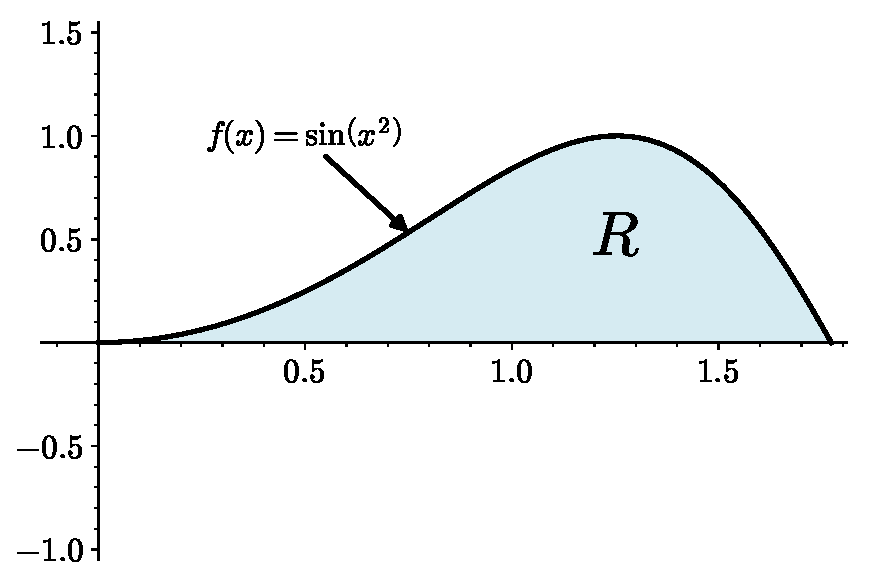
\includegraphics[scale=0.75]{plots/volume_by_shell_p1.pdf}
  \caption{Region bounded between $f(x)=\sin\lrp{x^2}$ and the $x$-axis}
\end{figure}

\part Draw the image that corresponds to unraveling the shell and label it.
\begin{solutionorbox}[\answerboxlengthone]
\end{solutionorbox}

\part What is the length of the shell?
\begin{solutionorbox}[\answerboxlengthone]
\end{solutionorbox}

\part What is the height of the shell?
\begin{solutionorbox}[\answerboxlengthone]
\end{solutionorbox}

\newpage 

\part What is the width of the shell?
\begin{solutionorbox}[\answerboxlengthone]
\end{solutionorbox}

\part Use this information to construct the Riemann sum that would calculate the volume of the solid of revolution.
\begin{solutionorbox}[\answerboxlengthone]
\end{solutionorbox}

\part Use your information from the previous part to construct and evaluate the definite integral that would calculate the volume of the solid of revolution.
\begin{solutionorbox}[4in]
\end{solutionorbox}

\end{parts}

\newpage
\question Let $R$ be the region shown in the figure below.

\begin{parts}
\newcommand\answerboxlengthone{1.20in}

\part Draw an example of a shell created by revolving a Riemann rectangle at $x_k^*$ in the interval $[0,2]$ about the line $x=3$.
\begin{figure}[hbt!]\centering
  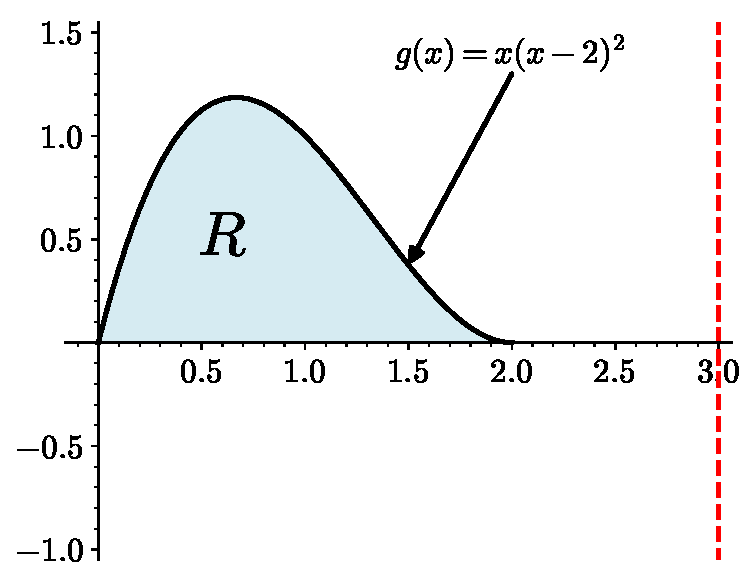
\includegraphics[scale=0.88]{plots/volume_by_shell_p2.pdf}
  \caption{Region bounded between $g(x)=x(x-2)^2$ and the $x$ axis}
\end{figure}

\part Draw the image that corresponds to unraveling the shell and label it.
\begin{solutionorbox}[\answerboxlengthone]
\end{solutionorbox}

\part What is the length of the shell?
\begin{solutionorbox}[\answerboxlengthone]
\end{solutionorbox}

\part What is the height of the shell?
\begin{solutionorbox}[\answerboxlengthone]
\end{solutionorbox}

\part What is the width of the shell?
\begin{solutionorbox}[\answerboxlengthone]
\end{solutionorbox}

\part Use this information to construct the Riemann sum that would calculate the volume of the solid of revolution.
\begin{solutionorbox}[\answerboxlengthone]
\end{solutionorbox}

\part Use your information from the previous part to construct and evaluate the definite integral that would calculate the volume of the solid of revolution.
\begin{solutionorbox}[4in]
\end{solutionorbox}

\end{parts}

\newpage
\question Find the volume of the solid created by rotating the region bounded by $y=x^2+2x-1$ and $y=2x$ about the line $x=-4$. Draw clearly labeled picture to support your answer.
\begin{solutionorbox}[9.25in]

\end{solutionorbox}

\question Find the volume of the solid created by rotating the region bounded by $y=\sin(x)+2$ and $y=\cos(x)$ on the interval $[0,\pi]$ about the line $x=6$.
\begin{solutionorbox}[9.25in]

\end{solutionorbox}



\end{questions}